\section{Website Structure}
The website is structure via a modified MVC pattern, for an explanation of the general idea of MVC see \secref{sec:mvc}.
In order to make the usage of MVC smooth, a framework was used \citep{misc:mvc-framework}.

The framework provides a controller base class that the new controllers inherit from, mainly providing a database instance.
It also provides an 'Application´ class that handles url parsing and navigation to the correct pages based on the url.
In addition to this, it provides a directory structure. As an example, you can add a controller to the controller directory, and the 'Application´ class is able to load them, same idea goes for the model and view layer.

\begin{figure}
	\centering
	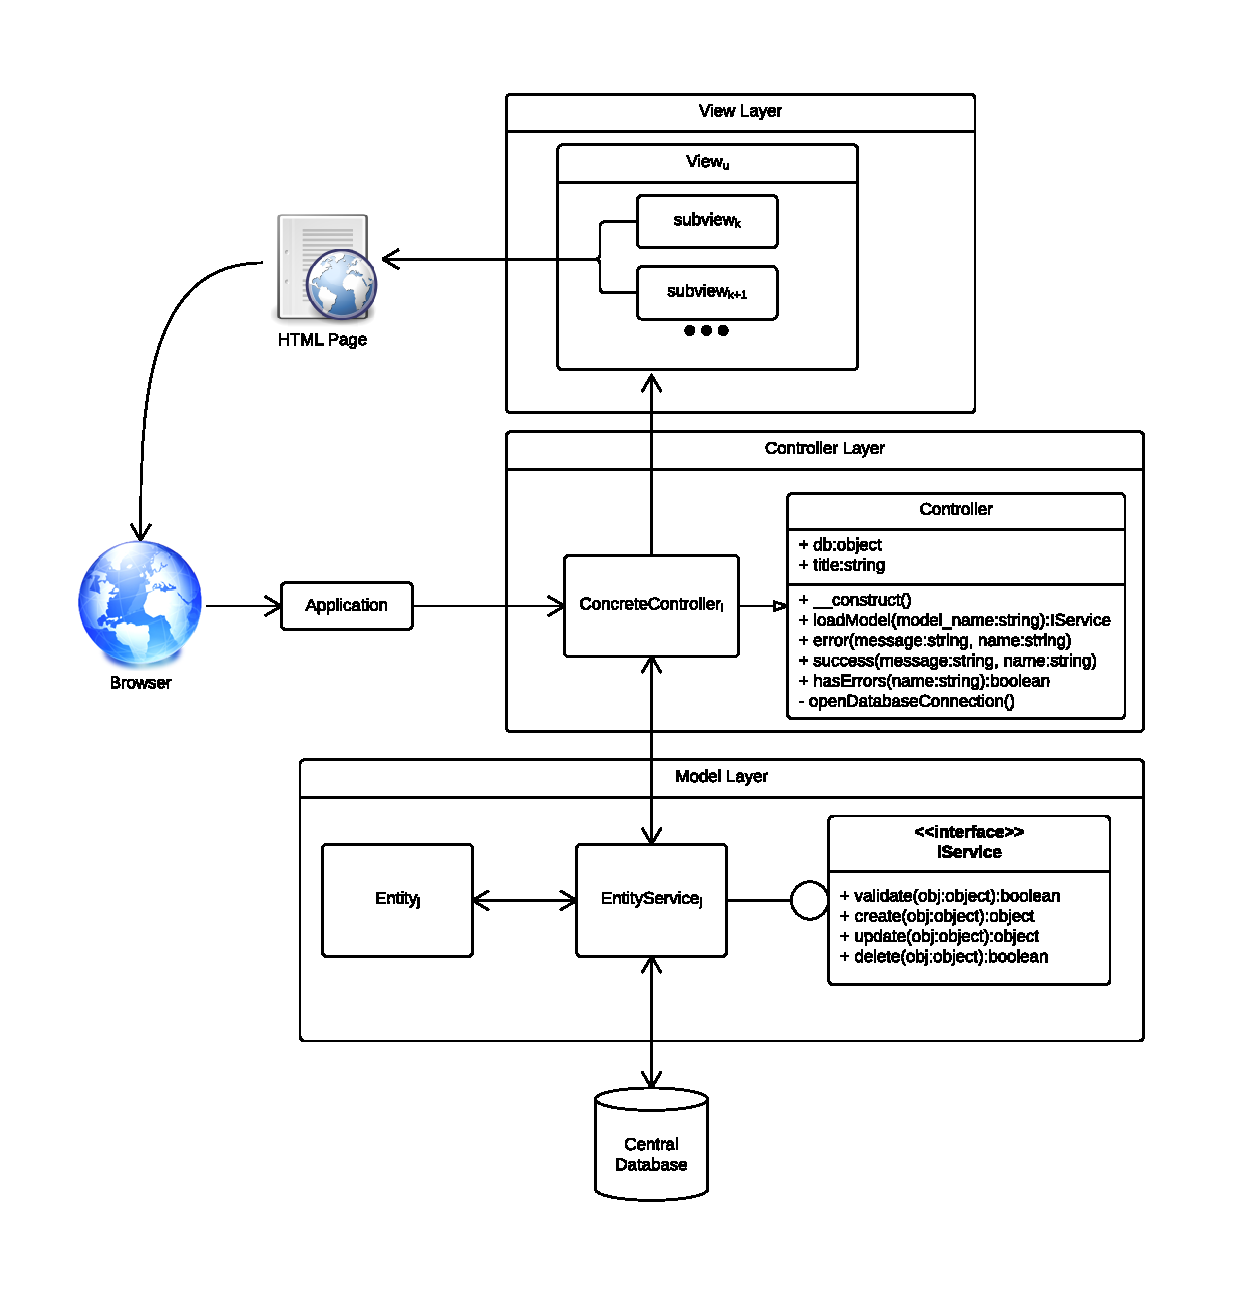
\includegraphics[scale=0.7, trim= 1cm 1.5cm 1.5cm 1.5cm, clip]{implementation/ConcreteMVC}
	\caption{Website Structure}\label{fig:websitestructure}
\end{figure}

With inspiration from the MVC pattern and usage of the framework, the website was then structured as seen in \figref{fig:websitestructure}.
The idea of the figure is to represent the structure, where we abstract from concrete entity, view, and controller names, and instead denote these with the names '$\text{Entity}_\text{j}$´, '$\text{EntityService}_\text{j}$´, '$\text{ConcreteController}_\text{i}$´, '$\text{View}_\text{u}$´.
The structure is split into several parts, each of which is examined in turn. 

\begin{description}[style=nextline]
	\item[Model Layer] 
	If you take a look at the model layer, it is split into three parts, $\text{Entity}_\text{j}$, $\text{EntityService}_\text{j}$ and iService.
	$\text{Entity}_\text{j}$ is a wrapper class, which is used to encapsulate a row from a table in the database.
	$\text{EntityService}_\text{j}$ is then a service, implementing the CRUD methods of iService, read is exluded from the interface as what amount of parameters you want to read with varies.
	$\text{EntityService}_\text{j}$ is what part of the model that then establishes the connection to the database, and enables the controller to work on the model, via calling the CRUD methods of the service, when a read method is called from a controller, an entity or a list of entities representing the row(s) is then what is returned.
	The reason we differentiate between  $\text{Entity}_\text{j}$ and $\text{EntityService}_\text{j}$ is that we found it makes sense to differentiate between the data and the methods working on the data, this is due to the work on the data is mainly reads, creations and deletions.\fxnote{er dette en god nok forklaring paa hvorfor vi differentierer?}
	
	\item[Controller Layer]
	The controller layer consists of a number of controllers $\text{ConcreteController}_\text{i}$, each of which inherits from a base Controller blass, which provides functionality to load the model as well as registering success' and errors to be displayed to the user by the view(s).
	Each Concrete controller then contains a number of functions, corresponding to different sites. The responsibility of the concrete controller is then to work on the model and include views. 
	
	\item[View Layer]
	The view layer takes care of the HTML generation part of the website, for each view included by the controllers, it consists of a number of subviews.
	By this we think of the combinations of subviews corresponding to a complete view, where some subviews occur in different views, e.g. header and footer subview.\fxwarning{ikke sikker paa dette er skrevet ordenligt}
	The combination of these subviews, the complete view, then takes care of representing a HTML page to be provided to the browser.
	
	\item[Application]
	When the browser visits the website, rewrite rules has been set in the \textit{.htaccess} file, to ensure that the relative path part of the url is given as an argument to the default index file. This index file then loads the required files, such that the thereafter instantiated Application object has access to the configuration files needed.
	The get variable url, which was set from the .htaccess file is then used by the Application object to navigate to the correct controller, which then takes care of the workflow to generate a htmlpage to the browser.
	
	
\end{description}

For a more detailed look at the model and controller layer, see \appref{app-arch:controller} and \appref{app-arch:model}.